\chapter{Crittografia classica}

\section{Cifrari simmetrici}
Con crittografia simmetrica, o crittografia a chiave privata, si intende una tecnica di cifratura che consiste nel cifrare
un testo in chiaro dove la chiave di crittazione è la stessa chiave di decrittazione. Non è previsto uno scambio di chiavi, 
dunque le due parti devono esserne già in
possesso.

\noindent Possiamo dividere i cifrari simmetrici in due categorie:
\begin{itemize}
    \item \textbf{Cifrari a flusso:} trasformano pochi bit alla volta (un singolo bit, o un byte); si rivelano adatti quando si deve 
    proteggere singoli dati generati uno dopo l'altro. Al flusso di dati in input in input corrisponde un \textit{flusso di chiavi}
    \item \textbf{Cifrari a blocchi:} trasformano blocchi di più bit (64, 128, o più); si rivelano adatti quando si devono 
    proteggere intere strutture dati 
\end{itemize}

\noindent Si può fare una distinzione tra due tecniche per la cifratura del testo in chiaro:
\begin{itemize}
    \item \textbf{Sostituzione:} i valori in chiaro vengono sostituiti con altri simboli
    \item \textbf{Trasposizione:} vengono scambiate le posizioni dei valori in chiaro 
\end{itemize}

\noindent Queste tecniche possono essere combinate tra loro, a patto che siano reversibili.

\subsection{Cifrari di shift}

Sono una generalizzazione del \textit{cifrario di Cesare}, senza fissare a 3 lo spostamento delle lettere.

\noindent Con questo approccio, lo schema di cifratura deve avere uno spazio delle chiavi non vulnerabile ad un attacco 
di \textit{forza bruta}; tuttavia, questa è una condizione necessaria ma non sufficiente!

\noindent Anziché semplicemente shiftare le lettere, si potrebbe effettuare una permutazione casuale delle lettere 
dell'alfabeto; la chiave, diventa dunque una stringa di 26 lettere.

\begin{figure}[H]
    \centering
    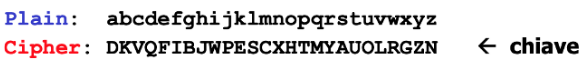
\includegraphics[width=0.7\linewidth]{chapters/chap2/images/shift.png}
\end{figure}

\noindent Con un alfabeto di 26 lettere, ci sono $26!$ possibili chiavi.

\noindent Potremmo aver pensato di aver ottenuto un adeguato livello di sicurezza, ma le caratteristiche del linguaggio naturale 
rendono possibili attacchi alternativi, come ad esempio la frequenza dei caratteri (che non cambia tra testo in chiaro e cifrato).

\noindent Alcune contromisure sono:
\begin{itemize}
    \item usare più simboli per cifrare i caratteri più frequenti, in modo da abbassare la frequenza 
    \item aggiungere simboli meno frequenti nel testo in chiaro, in modo da non compromettere il significato 
    \item usare parole in codice oltre ai simboli dell'alfabeto
\end{itemize}

\subsection{Cifrario affine}
Sono un caso particolare di cifrario a sostituzione monoalfabetico. Per trovare la sostituzione si usa un'espressione,
detta \textbf{affine}:

\begin{center}
    $c_i = E(p_i) = (k_1p_i + k_2) mod 26$
\end{center}

$\rightarrow$ la chiave è quindi data da \textbf{due costanti}.

\noindent La \textit{decrittazione} avviene invece secondo la formula:

\begin{center}
    $p_i = D(c_i) = (c_i - k_2) \cdot k_1^{-1}$
\end{center}

\noindent con $k_1^{-1}$ inteso come l'inverso modulo 26 di $k_1$, ovvero quel numero 
$x$ che soddisfa l'equazione:

\begin{center}
    $(k_1 \cdot x) mod 26 = 1$
\end{center}

\noindent Affinché questo sia possibile è necessario che $k_1$ e 26 siano primi tra loro.


\subsection{Cifrario Alberti}
Fu il primo meccanismo che usò più alfabeti cifranti che si sostituiscono durante la cifratura. Utilizza un apparecchio composto 
da due dischi concentrici, rotanti in maniera indipendente, contenenti un alfabeto ordinato per il testo in chiaro, ed uno disordinato per 
il testo cifrato.

\begin{figure}[H]
    \centering
    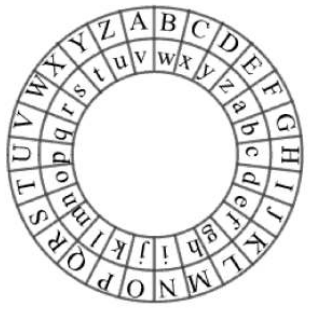
\includegraphics[width=0.4\linewidth]{chapters/chap2/images/disco.png}
\end{figure}

\noindent Si sceglie una lettera come chiave, la si fa corrispondere alla A del disco esterno, e per ogni lettera cifrata si muove 
in senso orario il disco interno.

\subsection{Cifrario Porta}

È un cifrario che si occupa di cifrare i \textbf{digrammi}, ovvero coppie di lettere. Ad ogni digramma viene assegnato un numero; la chiave 
è data da una permutazione arbitraria di numeri del cifrato e lettere su righe e colonne.

\begin{figure}[H]
    \centering
    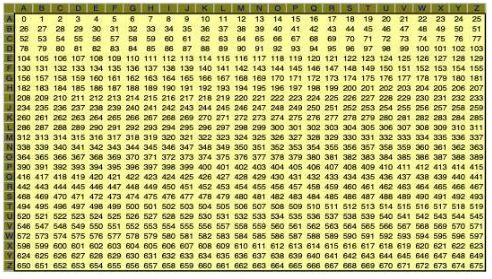
\includegraphics[width=0.8\linewidth]{chapters/chap2/images/porta.png}
\end{figure}

\subsection{Cifrario di Playfair}

È una tecnica di cifratura simmetrica manuale basata su un \textbf{cifrario monoalfabetico a due lettere} (vengono cifrate due 
lettere alla volta). L'analisi delle frequenze può ancora essere intrapresa, ma invece che 26 monografi esistono 
600 possibili digrafi! È dunque molto più difficile.

\noindent Il cifrario Playfair si basa sull'uso di una matrice $5 \times 5$ contenente una parola chiave; la tabella viene 
costruita inserendo le lettere della parola chiave senza lettere duplicate, per poi riempire gli spazi rimanenti con le lettere non utilizzate 
dell'alfabeto (in ordine).

\noindent Essendo disponibili 25 spazi, una lettera viene esclusa (di norma la Q o la W, oppure facendo collassare la I e la J nello 
stesso spazio). La chiave può essere scritta nelle celle della tabella seguendo una \textit{logica arbitraria}: la chiave è dunque 
\textbf{l'ordine di riempimento} della parola chiave nella tabella, oltre che la parola stessa.

\noindent La cifratura avviene separando le lettere del testo in chiaro in digrafi ed applicando a ciasuno di essi quattro regole:
\begin{enumerate}
    \item se entrambe le lettere sono uguali, si aggiunge una X (o una lettera poco comune) tra di loro e poi si ripete il procedimento 
    \item se le lettere appaiono nella stessa riga, vengono codificate con quelle alla propria destra 
    \item se le lettere appaiono nella stessa colonna, vengono codificate con quelle immediatamente sotto 
    \item altrimenti, si identifica un rettangolo che ha le due lettere come vertici opposti; le lettere vengono codificate con quella 
    sulla stessa riga in corrispondenza dell'altra colonna 
\end{enumerate}

\noindent Per decifrare, si usano regole inverse a queste.

\subsection{Cifrario di Hill}
Un cifrario a \textbf{sostituzione polialfabetica} basato sull'algebra lineare.
\begin{itemize}
    \item In \textit{primis}, viene fatto corrispondere ad ogni lettera un numero ($A=0, B=1, \dots$)
    \item Viene fissato un blocco di $n$ lettere, considerate come uno spazio vettoriale di dimensione $n$
    \item Il vettore ottenuto viene moltiplicato per una matrice $M$ di dimensione $n \times n$ in modulo 26 
    \item Segue che $m$ lettere in chiaro vengono sostituite con altrettante lettere cifrate secondo $m$ equazioni lineari 
\end{itemize}
\noindent La chiave è data dalla matrice $M$; deve essere casuale a patto che sia invertibile in $\mathbb{Z}_26 $ affinché la 
decrittazione sia possibile.

\noindent Ad esempio, il messaggio \texttt{TUO} verrebbe cifrato con la chiave \texttt{YYPRZWIZJ} come:

\begin{figure}[H]
    \centering 
    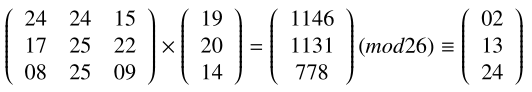
\includegraphics[width=0.5\linewidth]{chapters/chap2/images/hill.png}
\end{figure}

\subsection{Cifrario di Vigenère}

È un il più semplice tra i cifrari \textbf{polialfabetici}, è considerabile come una \textbf{generalizzazione del cifrario di Cesare}: invece 
di spostare sempre dello stesso numero di posti la lettera da cifrare, essa viene spostata di un numero di posti variabile, ma ripetuto, 
determinato attraverso una \textbf{parola chiave}.

\noindent Rispetto ai cifrari monoalfabetici, si ha il \textit{vantaggio} di avere $n$ alfabeti cifranti ($n$ lunghezza della chiave). La 
\textit{debolezza} consiste che si tratta di $n$ cifrari di Cesare, motivo per cui è possibile, a partire dalle ripetizioni, stimare la 
lunghezza della chiave per poi analizzare le frequenze in ognuno degli alfabeti cifranti.

\subsection{Cifrario di Vernam}
È un cifrario di Vigenère a cui viene imposto che la chiave abbia la stessa lunghezza del messaggio da cifrare.

\noindent Questo metodo è potenzialmente \textbf{\textit{unconditionally secure}} (ossia sicuro indipendentemente dal tempo e risorse), ma 
ha il problema di necessitare di una chiave casuale (già di per sé difficile siccome le chiavi sono pseudo-casuali) ed eventualmente di grandi 
dimensioni.


